\section{Theoretical Model} \label{sec:Theoretical Model}
    For better understanding of the computational and experimental components of this paper, we will first establish a number of mathematical preliminaries, to better visualize the question at hand. Firstly, we will maintain the coordinate system in Figure 1, with the "x" direction being along a door (pointing from the hinges towards the knob of an unperturbed door), the (x,y) plane being that of the ground, and the "z" direction being upwards through the hinges. Any "observer" will be in reference to that person making the decision of which door to choose, and any "initializer" will be in reference to that person releasing the door, entering immediately prior to the observer. Further, let " $\vec{v}$ " be the velocity in the y-direction of the observer towards the door, let "d" be the distance between the observer and the initializer, and let "l" and "m" be the length and mass of the door, respectively. Finally, it follows that the time required for the observer to arrive at the set of doors is found by:
    \begin{eqnarray}
        v=\frac{d}{t_{0}}\Rightarrow{}t_{0}=\frac{d}{v}
    \end{eqnarray}.
    \par
    Next we must determine at what point the observer will be able to pass through the door, as surely we should not expect the observer to contort themself beyond reason. Now, the point at which a person's breadth is maximized varies (certainly on individual bases, but categorically speaking, specific groups tend to see this maximization around predominantly either the hips or the shoulders), but on average this breadth hovers around or below 40cm as found in [1]. Added to a buffer of around 10cm on each side, we will call this breadth the opening distance: $"d_{0}"\approx60cm.$ Because our door -opened to any point-, the base of the unperturbed door, and our opening distance act as sides of a triangle,in fact an isosceles triangle, we may apply the law of cosines:
    
    \begin{eqnarray}
    \begin{split}
        d_{0}^{2} & =a^{2}+b^{2}-2ab\cos(\theta_{req}) \\
        & = 2l^{2}-2l^{2}\cos(\theta_{req})
    \end{split}
    \theta_{req}=\cos^{-1}(1-\frac{d_{0}^{2}}{2l^{2}}).
    \end{eqnarray}
    Here, $\theta_{req}$ is the required angle from the x-axis in the (x,y) plane which the door must point for the observer to comfortably pass through, displayed in Figure 2(c). \par
    \begin{figure}[htp]
    \centering
    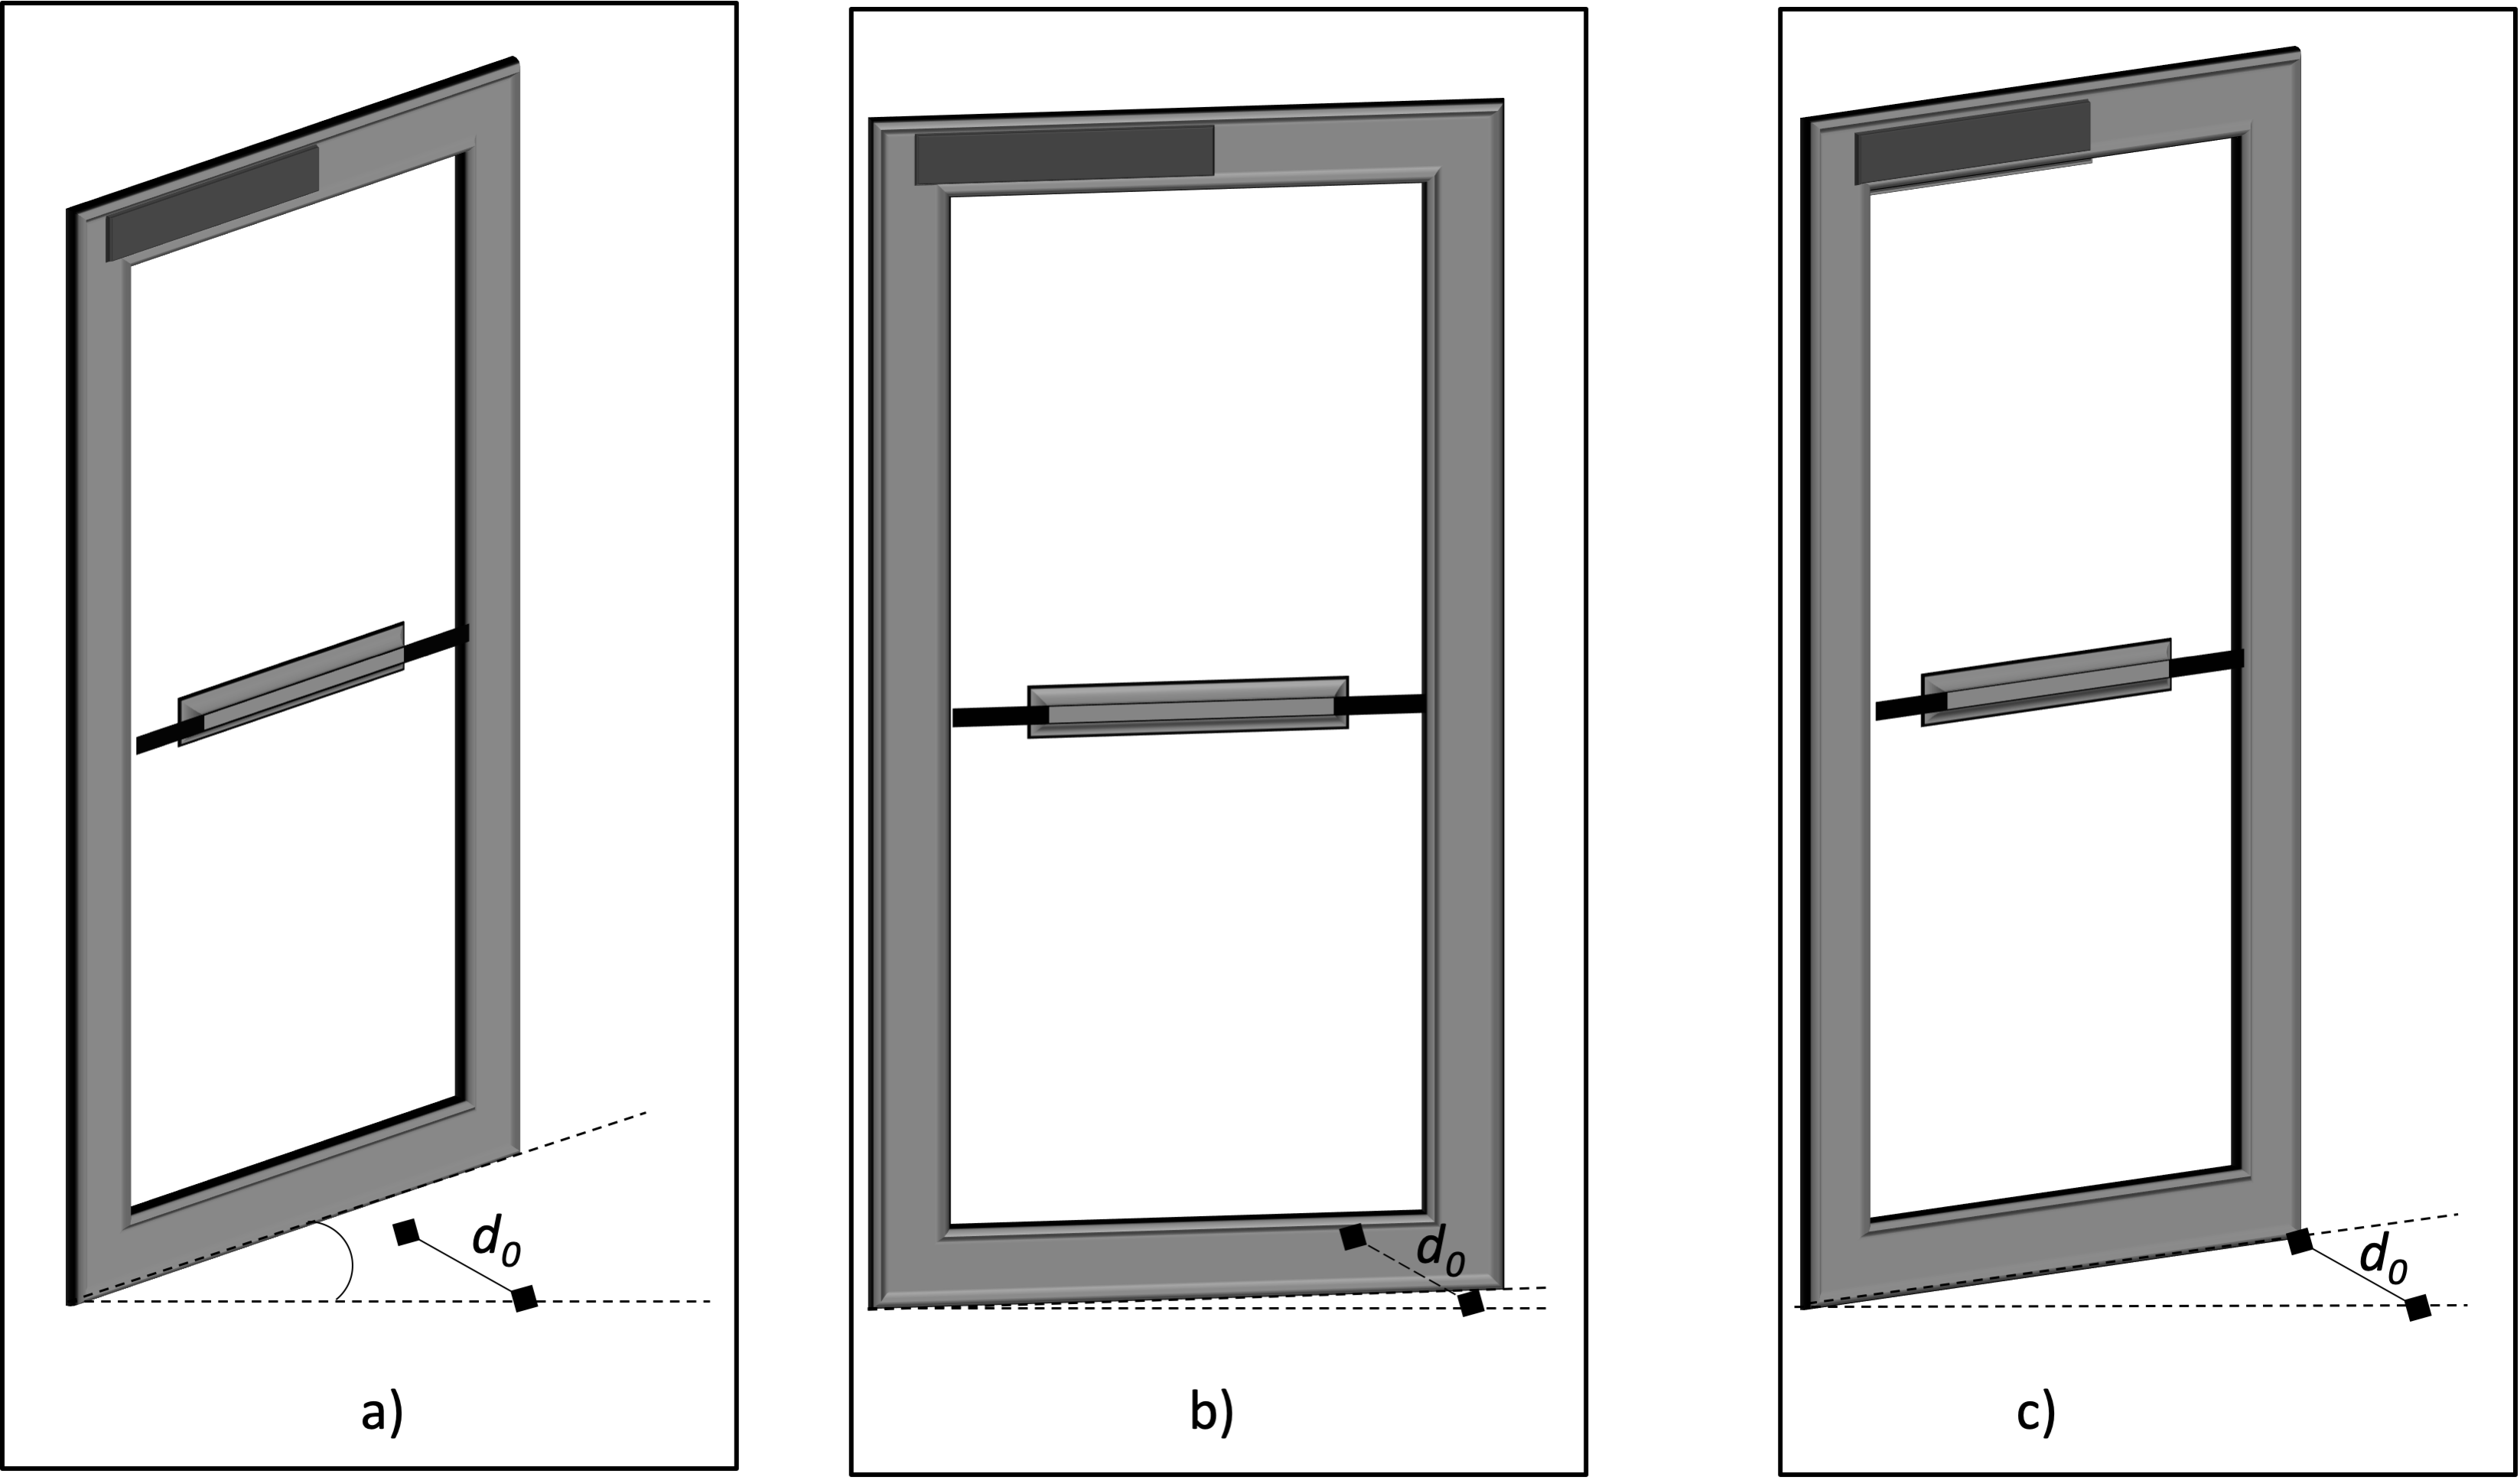
\includegraphics[width=\linewidth]{figures/Figure 2 - Angles.png}    
    \caption{A schematic showing a door opened to various angles. a) $\theta>\theta_{req}$, b) $\theta<\theta_{req}$, c) $\theta=\theta_{req}$. Also, $d_{0}$ is displayed, being the comfortable opening distance discussed.}
    \end{figure}
    We turn now to the primary question at hand, pertaining to the work required of the observer. Namely, for a force applied by the observer $\vec{F}$, perpendicular to a door pointing at some initial angle $\theta_{0}$, :
    \begin{eqnarray}
    \begin{split}
        W & =\int \Vec{F}\cdot \,\vec{dl_{\theta}}\\
        & =\int_{\theta_{0}}^{\theta_{req}} F\cdot l \,d\theta\\
        & = Fl(\theta_{req}-\theta_{0})\\
        & = \tau (\theta_{req}-\theta_{0})
    \end{split}.
    \end{eqnarray} \par
    Now, $\tau$ is some torque in the z-direction, which can be extracted from the angular impulse relation if we allow for some relatively short time $t_{impulse}$ (say 0.5s). Let the initial angular velocity of the door $\vec{\omega_{0}}$ be equal to the angular velocity of the door at time $t_{0}$ and let the final angular velocity be given by:
    \begin{eqnarray}
    \begin{split}
        \vec{\omega_{f}} & = \frac{\vec{r} \cross \vec{v}}{\norm{r}^{2}}\\
        & = \frac{v}{l},
    \end{split}
    \end{eqnarray}
    the former of which will be derived for the cases in the following subsections. Note, then that the angular momenta are:
    \begin{eqnarray}
    \begin{split}
        L_{0}=I\vec{\omega_{0}}=I\omega_{0,z}, \text{ and }  L_{f}=I\vec{\omega_{f}}=\frac{Iv}{l},
    \end{split}
    \end{eqnarray}
    and thus,
    \begin{eqnarray}
    \begin{split}
        \Delta L & = L_{f}-L_{0} = \frac{Iv}{l}-I\omega_{0,z}=\\
        & = I(\frac{v}{l}-\omega_{0,z})=\tau t_{impulse},
    \end{split}\\
    \begin{split}
        \tau & =\frac{I}{t_{impulse}}(\frac{v}{l}-\omega_{0,z}).
    \end{split}
    \end{eqnarray}\par
    Further, if we consider the door to have a uniform mass distribution $\rho=\frac{m}{l}$ and to be rotating about the hinges, we have that
    \begin{eqnarray}
    \begin{split}
        I & =\int_{0}^{l} \rho r^{2} \,dr = \frac{1}{3} \rho r^{3} |_{0}^{l}=\frac{1}{3}\frac{m}{l}l^{3}\\
        & = \frac{1}{3}ml^{2}.
    \end{split}
    \end{eqnarray}
    Thereby, we can substitute equations (8) and (9) into equation (4) to find:
    \begin{eqnarray}
    \begin{split}
        W & =\frac{1}{3}\frac{ml^{2}}{t_{impulse}} (\theta_{req}-\theta_{0}) (\frac{v}{l}-\omega_{0,z}).
    \end{split}
    \end{eqnarray}
    Note that the units are consistent with units of work. Also note that, as expected, if $\theta_{0}>\theta_{req}$ then the work is negative, being that any further energy exerted by the observer would not make it any easier to comfortably fit through the door. Finally, note that the work needed to open the unopened door to the required angle (i.e. when both $\omega_{0,z}$ and $\theta_{0}$ are identically 0) is given by:
    \begin{eqnarray}
    \begin{split}
        W & = \frac{1}{3}\frac{mlv}{t_{impulse}}.
    \end{split}
    \end{eqnarray}\par
    We will next consider Undamped, as well as Critically and Overdamped manual door closers, and in specific, derive the $\omega_{0,z}$ defined in this problem for each case. We will additionally do this for an Underdamped case, in a similar problem involving a double hinged door.
    \subsection{Undamped Case}
    For each of these cases, one might find it helpful to envision a common mass-spring system, or simple pendulum; and particularly, review of of references [2] and [3] could prove useful. Here, at $t=0$ we have that the door has been released by the initializer, and the manual door closer has begun to move the door back towards it's equilibrium position. Let the angular acceleration describing the door's motion be $a_{\theta}=l\ddot\theta$, and let the torque of the manual door mover be $\tau_{m}=-\kappa\theta$, where $\kappa$ is some torsion coefficient. The force on the door can thus be found:
    \begin{eqnarray}
    \begin{split}
        \tau & = \vec F \cdot \vec r = F(\theta)l = -\kappa \theta,
    \end{split}
    \begin{split}
        F(\theta) & = -\frac{\kappa}{l}\theta,
    \end{split}
    \end{eqnarray}
    which will be equivalent to the sum of all forces acting on the door, $\sum F$, while $t\in[0,t_{0}]$.\par
    We then have, by Newton's second law:
    \begin{eqnarray}
    \begin{split}
        ma_{\theta}=F(\theta)\\
        ml\ddot\theta = -\frac{\kappa}{l}\theta\\
        ml\ddot\theta+\frac{\kappa}{l}\theta=0\\
        \ddot\theta + \frac{\kappa}{ml^{2}}\theta=0.
    \end{split}
    \end{eqnarray}
    To avoid confusion with the above formalism, we will define the constant $c^{2}\equiv\frac{\kappa}{ml^{2}}$ (instead of the commonly used $\omega_{0}^{2}$). We then have that (13) is a second order ordinary differential equation with solution:
    \begin{eqnarray}
    \begin{split}
        \theta(t)=A\cos(ct+\phi),
    \end{split}
    \end{eqnarray}
    where A and $\phi$ are constants.\par
    To determine these constants, we must have the angle at which the initializer releases the door and at what angular velocity they release it at, call them $\theta(0)\equiv\theta_{i}$ and $\dot\theta(0)\equiv\dot\theta_{i}$, respectively. We can then use (14) and the fact that
    \begin{eqnarray}
    \begin{split}
        \dot\theta(t)=\frac{d}{dt}A\cos(ct+\phi)=-Ac\sin(ct+\phi)
    \end{split}
    \end{eqnarray}
    to see that
    \begin{eqnarray}
    \begin{split}
        \cos^{2}(\phi) = \frac{\theta_{i}^{2}}{A^{2}} \text{ and }
        \sin^{2}(\phi)=\frac{\dot\theta_{i}^{2}}{c^{2}A^{2}}
    \end{split}\\
    \end{eqnarray}
    so that
    \begin{eqnarray}
    \begin{split}
        A^{2}=\theta_{i}^{2}+\frac{\dot\theta_{i}^{2}}{c^{2}}, \text{ or }
        A=\sqrt{\theta_{i}^{2}+\frac{\dot\theta_{i}^{2}}{c^{2}}},
    \end{split}
    \end{eqnarray}
    and using (17) in (14), we have that 
    \begin{eqnarray}
    \begin{split}
        \phi=\frac{\theta_{i}}{\sqrt{\theta_{i}^{2}+\frac{\dot\theta_{i}^{2}}{c^{2}}}}
    \end{split}.
    \end{eqnarray}\par
    Finally, from (15), we can find the angular velocity for our considered problem:
    \begin{eqnarray}
    \begin{split}
        \omega_{0,z} & = \dot\theta(t_{0})=-Ac\sin (ct_{0}+\phi)
    \end{split}.
    \end{eqnarray}
    and equation (9) becomes
    \begin{eqnarray}
    \begin{split}
        W & =\frac{1}{3}\frac{ml^{2}}{t_{impulse}}(\theta_{req}-\theta_{0}) (\frac{v}{l}+Ac\sin(ct_{0}+\phi)),
    \end{split}
    \end{eqnarray}
    with each of the constants as previously defined. \\
    \subsection{Damped Cases}
    Though the undamped case is certainly interesting, it hardly can be applied generally to the situation at hand. In fact, the undamped case would be better suited for something like a door which closes using a spring (similar to the way a mouse/rat trap might close), rather than the typical manual closer found commonly throughout everyday life. It is thus necessary to consider the case of dampened manual door closers, and their impact on our problem.\par
    We start similarly that of the undamped case, by calling the same $a_{\theta}$ and $F(\theta)$, however this time, the sum of the forces acting on the door will have an additional angular-velocity-limiting factor:
    \begin{eqnarray}
    \begin{split}
        \sum F & = \alpha\vec v_{\tan,door} + F(\theta) = -bl\dot\theta-\frac{\kappa}{l}\theta
    \end{split}.
    \end{eqnarray}
    Equation (12) then becomes
    \begin{eqnarray}
    \begin{split}
        \ddot\theta+\frac{b}{m}\dot\theta+\frac{\kappa}{ml^{2}}\theta=0
    \end{split},
    \end{eqnarray}
    and if we allow again the constant $c^{2}\equiv\frac{\kappa}{ml^{2}}$ and replace $\frac{b}{m}\equiv2\beta$, the corresponding general solution of (23) is
    \begin{eqnarray}
    \begin{split}
        \theta(t)=e^{-\beta t}(A_{1}e^{\sqrt{\beta^{2}-c^{2}}t}+A_{2}e^{-\sqrt{\beta^{2}-c^{2}}t})
    \end{split}.
    \end{eqnarray} \par
    We thus have three cases, as per usual:
    $\beta^{2}>c^{2}$, called overdamping, in which case the square roots are real and the corresponding equation is a decaying exponential; $\beta^{2}=c^{2}$, called critically damping, which also results in a decaying exponential, though it has no buffer and goes to zero much faster than the overdamped case; and $\beta^{2}<c^{2}$, called underdamping, in which case the square roots are imaginary, and the resulting equation resembles that of a cosine function. Note that the underdamped case, if the door is single hinged, will act similarly to that of the undamped case (in that they both are resembling cosine functions), though with a decaying factor "tacked on". We will develop this resemblance further in our discussion of the double hinged door, as well as determine the $\omega_{0,z}$ for each case.\\
    \subsubsection{Overdamped and Critically-damped Cases}
    For the Overdamped case, we begin with defining a $c_{0}=\sqrt{\beta^{2}-c^{2}}$, so that (23) will become
    \begin{eqnarray}
    \begin{split}
        \theta(t)=e^{-\beta t}(A_{1}e^{c_{0}t}+A_{2}e^{-c_{0}t})
    \end{split}.
    \end{eqnarray}
    Now we may find the angular velocity at time $t_{0}$:
    \begin{eqnarray}
    \begin{split}
        \omega_{0,z} & =\dot\theta(t_{0})\\
        & =(A_{1}(c_{0}t+\beta)e^{2c_{0}t}+A_{2}(c_{0}-\beta))e^{-t(c_{0}-\beta)}.
    \end{split}
    \end{eqnarray}
    Here, we have:
    \begin{eqnarray}
    \begin{split}
        \theta(0)=\theta_{i}=A_{1}+A_{2}, \text{ as well as }\\ \dot\theta(0)=\dot\theta_{i}=A_{1}\beta+A_{2}(c_{0}-\beta),
    \end{split}
    \end{eqnarray}
    and with some algebraic manipulation, we find
    \begin{eqnarray}
    \begin{split}
        A_{2}=\frac{\beta\theta_{i}-\dot\theta_{i}}{2\beta-c_{0}}, \text{ and }
        A_{1}=\theta_{i}-\frac{\beta\theta_{i}-\dot\theta_{i}}{2\beta-c_{0}}
    \end{split}.
    \end{eqnarray}
    It would then suffice to insert (26) into (9) to determine a solution to our problem.\par
    Next, for the critically damped case, we have that our $c_{0}^{2}=\beta^{2}$. Here, the solution to (23) is not (24), but rather the general solution for a repeated root:
    \begin{eqnarray}
    \begin{split}
        \theta(t)=e^{-\beta t}(A+Bt)
    \end{split},
    \end{eqnarray}
    and our angular velocity at time $t_{0}$ is
    \begin{eqnarray}
    \begin{split}
        \omega_{0,z}=\dot\theta(t_{0})=e^{-\beta t_{0}}(B(1-\beta t_{0})-A\beta)
    \end{split}.
    \end{eqnarray}
    We can use our initial conditions to find the constants A and B:
    \begin{eqnarray}
    \begin{split}
        \theta(0)=\theta_{i}=A, \text{ and }\\
        \dot\theta(0)=\dot\theta_{i}=B-A\beta, \text{ or } B=\dot\theta_{i}+\theta_{i}\beta,
    \end{split}
    \end{eqnarray}
    and similarly to the overdamped case, insert (30) into (9) to gather a solution to our problem. 
    \subsubsection{Underdamped Case (double-hinged doors)}
	For the Under-damped Case, we define $c_{0}=\sqrt{\beta^{2}-c^{2}}$, as $\beta^{2}-c^{2}<0$, then we can rewrite $c_{0}=\sqrt{c^2-\beta^{2}}i$. So that (24) will become
    \begin{eqnarray}
    \begin{split}
      \theta(t)=e^{-\beta t}(A_{1}e^{c_{0}t}+A_{2}e^{-c_{0}t})
    \end{split}
    \end{eqnarray}
    Now we find the angular velocity at time t0:\begin{eqnarray}
    \begin{split}
        \omega_{0,z} & =\dot\theta(t_{0})\\
        & =(A_{1}(c_{0}t+\beta)e^{2c_{0}t}+A_{2}(c_{0}-\beta))e^{-t(c_{0}-\beta)}.
    \end{split}
    \end{eqnarray}
    Here, we have :
      \begin{eqnarray}
    \begin{split}
        \theta(0)=\theta_{i}=A_{1}+A_{2}, \text{ as well as }\\ \dot\theta(0)=\dot\theta_{i}=A_{1}\beta+A_{2}(c_{0}-\beta),
    \end{split}
    \end{eqnarray}  and with some algebraic manipulation, we find
    
    \begin{eqnarray}
    \begin{split}
        A_{2}=\frac{\beta\theta_{i}-\dot\theta_{i}}{2\beta-c_{0}}, \text{ and }
        A_{1}=\theta_{i}-\frac{\beta\theta_{i}-\dot\theta_{i}}{2\beta-c_{0}}
    \end{split}.
    \end{eqnarray}
      It would then suffice to insert (34) into (9) to determine a solution to our problem.\par

    
